
% !TeX root=first.tex

\section{Praktische Vorstellung der Personaladministration}
\label{sec:praktischevorstellungderpersonaladministration}

\subsection{Einstellungsprozess}
\subsubsection{Anlegen einer Planstelle}
Eine Planstelle wird von Mitarbeitern besetzt und ist einer Organisationseinheit zugeordnet. Eine Planstelle ist beispielsweise ein Sachbearbeiter und die zugehörige Organisationseinheit ist die Kreditorenbuchhaltung. Um eine neue Planstelle anzulegen, Anlegewird die Anwendung „Organisation und Besetzung ändern“ gestartet.

\begin{figure}[H]
	\centering
	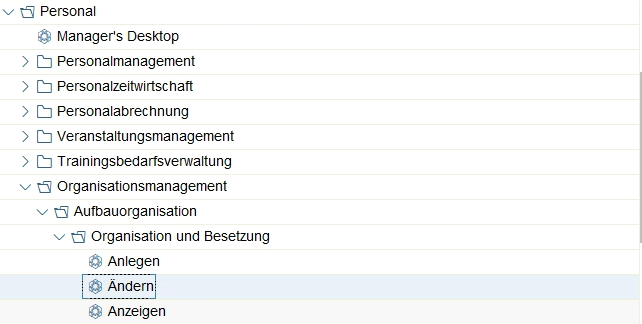
\includegraphics[scale=0.7]{pfad_planstelleanlegen}
	\caption{Pfad der Planstellenanlage}
	\label{fig:pfad_planstelleanlegen}
\end{figure}

Die Planstelle wird in der Abteilung „Security“ angelegt. Die Organisationseinheit wird mit der integrierten Suchfunktion über den Begriff „038 Security“ gesucht. Mit einem Doppelklick wird die Organisationseinheit geöffnet. Über die Funktion „anlegen“ wird eine neue Planstelle für die Organisationseinheit angelegt.

\begin{figure}[H]
	\centering
	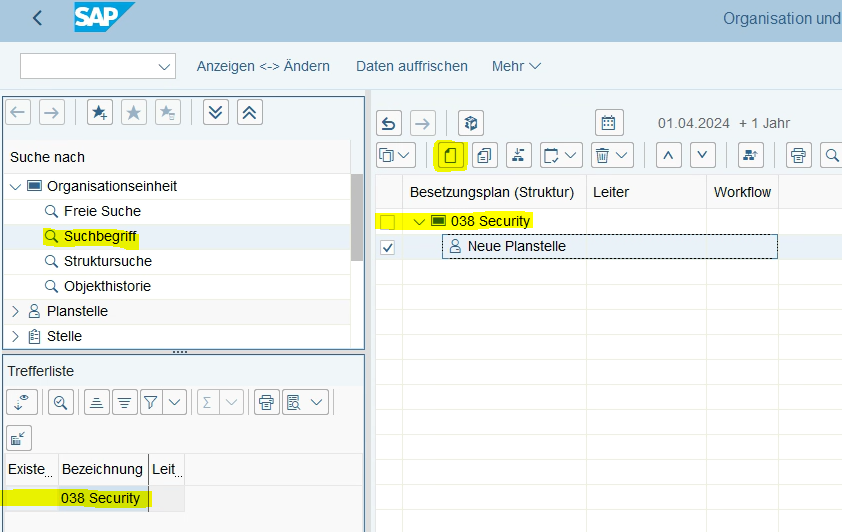
\includegraphics[scale=0.6]{anlegen_planstelle}
	\caption{Anlegen der Planstelle}
	\label{fig:anlegen_planstelle}
\end{figure}

Im unteren Bereich werden Detaildaten für die neue Positionen gepflegt. Hier wird die Planstelle „038 CSM“ und die Bezeichnung „038 Chief Security Manager“ gepflegt und als „Leiter der eigenen Organisationseinheit“ markiert.

\begin{figure}[H]
	\centering
	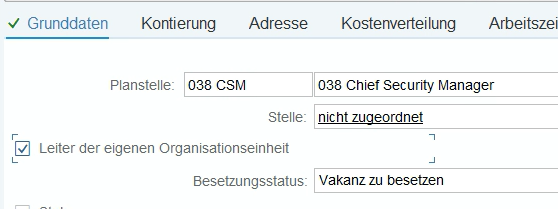
\includegraphics[scale=0.6]{planstelle_pflegen}
	\caption{Pflegen der Planstelle}
	\label{fig:planstelle_pflegen}
\end{figure}

Mit dem gleichen Vorgehen werden nun die Planstellen „038 SG“ mit der Bezeichnung „038 Security Guard“ und „038 SM“ mit der Bezeichnung „038 Security Manager“ angelegt. Allerdings werden die beiden neuen Planstellen nicht als „Leiter der eigenen Organisationseinheit“ markiert. Der Besetzungsplan hat danach folgende Struktur:

\begin{figure}[H]
	\centering
	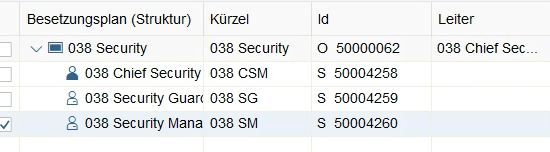
\includegraphics[scale=0.6]{struktur_besetzungsplan}
	\caption{Besetzungsplan Struktur}
	\label{fig:struktur_besetzungsplan}
\end{figure}

\subsubsection{Anlegen der Laufbahn}
In der Abbildung wird der Pfad für das Anlegen der Laufbahn dargestellt.

\begin{figure}[H]
	\centering
	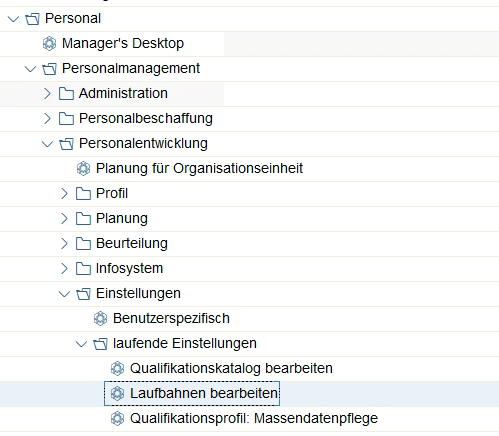
\includegraphics[scale=0.6]{pfad_laufbahnanlegen}
	\caption{Pfad Laufbahn bearbeiten}
	\label{fig:pfad_laufbahnanlegen}
\end{figure}

Über die Funktion „Anlegen“ wird die Laufbahn „038 Security Guard“ angelegt.

\begin{figure}[H]
	\centering
	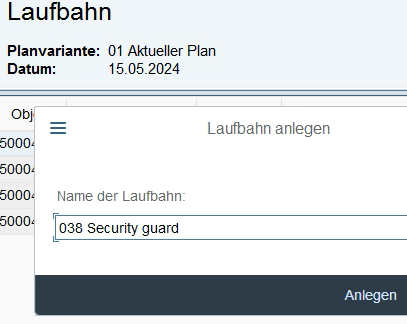
\includegraphics[scale=0.6]{anlegen_laufbahn}
	\caption{Laufbahn anlegen}
	\label{fig:anlegen_laufbahn}
\end{figure}

Um den grafischen Editor zum Anlegen von Laufbahnen zu öffnen, wird die Laufbahn „038 Security Guard“ ausgewählt und geöffnet mit dem Button „Ändern“. Mit dem grafischen Editor wird es ermöglicht eine Laufbahn in Form eines Netzplans anzulegen. Im „Knotenbereich“ wird die „Planstelle“ in den „Anzeigebereich“ hinzugefügt. Daraufhin öffnen sich die Suche für die Planstelle.

\begin{figure}[H]
	\centering
	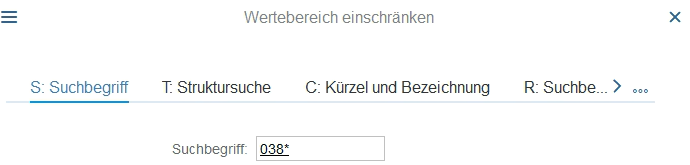
\includegraphics[scale=0.6]{suche_planstelle}
	\caption{Planstelle suchen}
	\label{fig:suche_planstelle}
\end{figure}
\begin{figure}[H]
	\centering
	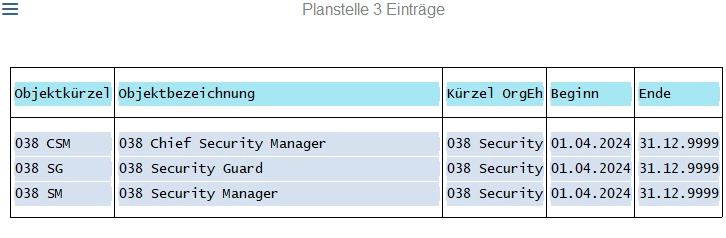
\includegraphics[scale=0.6]{suche_planstelle2}
	\caption{Planstelle suchen 2}
	\label{fig:suche_planstelle2}
\end{figure}

Es wird die Planstelle „038 Chief Security Manager“ als gelbes Rechteck im Anzeigebereich ausgegeben. Danach wird mit dem gleichen Verfahren die nächste Planstelle „038 Security Manager“ hinzugefügt.
\begin{figure}[H]
	\centering
	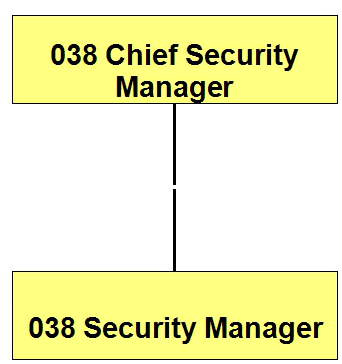
\includegraphics[scale=0.6]{knoten_securitymanager}
	\caption{Knoten von 2 Planstellen}
	\label{fig:knoten_securitymanager}
\end{figure}
Mit einem Doppelklick auf die neu hinzugefügte Planstelle wird die Pflegedauer auf 5 Jahre festgelegt. Mit dem gleichen Vorgehen wird die nächste Planstelle „038 Security Guard“ mit einer Pflegedauer von 3 Jahren definiert.
\begin{figure}[H]
	\centering
	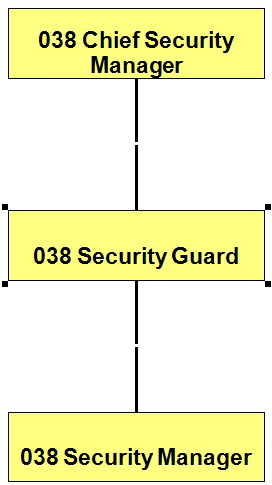
\includegraphics[scale=0.6]{grafisch_laufbahn}
	\caption{Knoten von 3 Planstellen}
	\label{fig:grafisch_laufbahn}
\end{figure}

\subsubsection{Festlegen Anforderung}
Eine Anforderung für eine Planstelle wird in der Anwendung „Profil ändern“ definiert.
\begin{figure}[H]
	\centering
	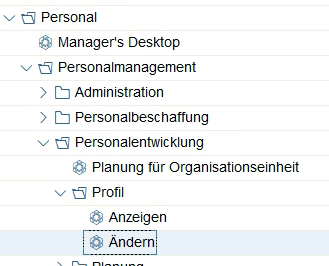
\includegraphics[scale=0.6]{profil_aendern}
	\caption{Pfad Profil ändern}
	\label{fig:profil_aendern}
\end{figure}
Es wird nach den angelegten Planstellen mit „038*“ gesucht, um mit einem Doppelklick auf die Planstellen in das Kontextmenü für die Anforderung zu gelangen. Hier wird die Anforderung für die Planstelle „038 Security Manager“ definiert. Es werden die Qualifikationen „First Aid Certification“ und „GIAC Security Leadership Certification“ ausgewählt.
\begin{figure}[H]
	\centering
	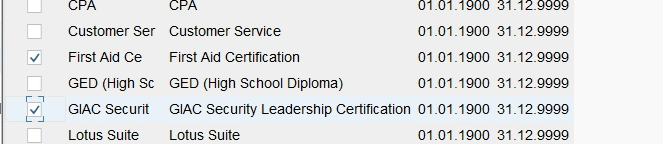
\includegraphics[scale=0.6]{qualifikationen_anforderung}
	\caption{Qualifikationen auswählen}
	\label{fig:qualifikationen_anforderung}
\end{figure}
Die Anforderungen werden in einer Liste angezeigt.
\begin{figure}[H]
	\centering
	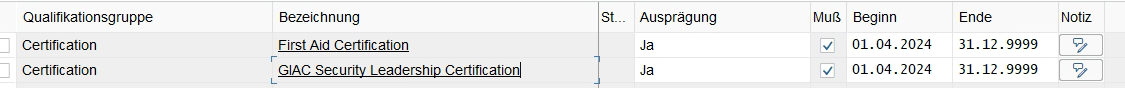
\includegraphics[scale=0.4]{liste_anforderung}
	\caption{Liste der Anforderung}
	\label{fig:liste_anforderung}
\end{figure}

\subsubsection{Einstellen der Mitarbeiter}
Um einen Mitarbeiter einzustellen wird die Anwendung „Personalmaßnahmen" geöffnet.
\begin{figure}[H]
	\centering
	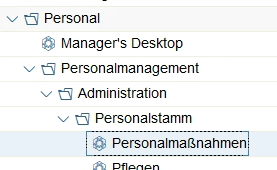
\includegraphics[scale=0.6]{pfad_personalmassnahmen}
	\caption{Pfad der Personalmaßnahmen}
	\label{fig:pfad_personalmassnahmen}
\end{figure}
Es wird die „Einstellung (Reise-Ministamm)“ mit dem Personalbereich „GBI Dallas“, Mitarbeitergruppe als „Aktive“ und Mitarbeiterkreis als „Angestellte“ gepflegt und ausgeführt.
\begin{figure}[H]
	\centering
	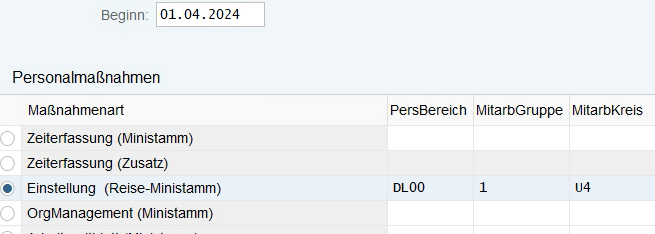
\includegraphics[scale=0.6]{pflege_personalmassnahmen}
	\caption{Pflege der Personalmaßnahmen}
	\label{fig:pflege_personalmassnahmen}
\end{figure}
In der organisatorischen Zuordnung wird die Planstellen ID der Planstelle „038 Chief Security Manager“ gepflegt.
\begin{figure}[H]
	\centering
	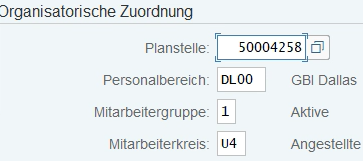
\includegraphics[scale=0.6]{zuordnung_planstelle}
	\caption{Zuordnung der Planstelle}
	\label{fig:zuordnung_planstelle}
\end{figure}
Die automatisch angelegte Personalnummer ist die 1083. Es werden die Anrede, Vor- und Nachnamen, das Geburtsdatum und die Sozialversicherungsnummer befüllt.
\begin{figure}[H]
	\centering
	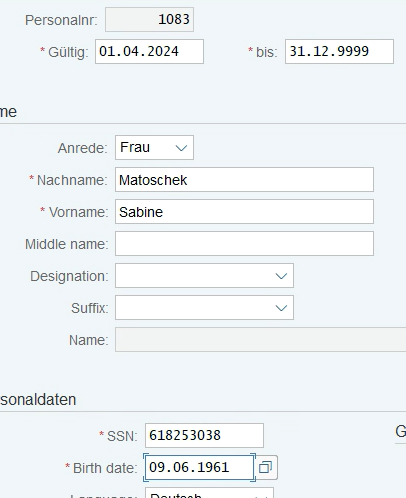
\includegraphics[scale=0.6]{pflege_sabine}
	\caption{Pflege des Chief Security Manager}
	\label{fig:pflege_sabine}
\end{figure}
Im darauffolgenden Bereich wird in der Unternehmensstruktur der Personalteilbereich mit „EX00“ definiert und gesichert. Der Subtyp der Anschrift wird als „Ständiger Wohnsitz ausgewählt. In der Anschrift wird die Straße „Betonanienstrasse 45“, Ort „Dallas“, Bundesstaat „TX“ und Postleitzahl „75201“ definiert.
\begin{figure}[H]
	\centering
	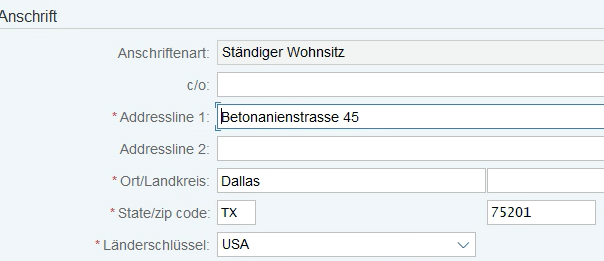
\includegraphics[scale=0.6]{anschrift_sabine}
	\caption{Pflege der Anschrift von Sabine}
	\label{fig:anschrift_sabine}
\end{figure}
Im darauffolgenden Dialog wird das Steuergebiet Texas ausgewählt. Die nächsten beiden Infotypen werden ohne weitere Änderungen gesichert.

\subsection{Rekrutierungsprozess}

\subsubsection{Ausschreiben der Stelle}
Um eine Stellenausschreibung anzulegen, wird die Anwendung „Ausschreibung pflegen“ gestartet.
\begin{figure}[H]
	\centering
	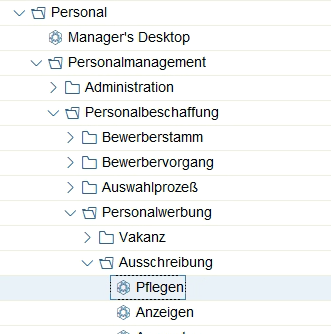
\includegraphics[scale=0.6]{pflegen_ausschreibung}
	\caption{Pfad Ausschreibung pflegen}
	\label{fig:pflegen_ausschreibung}
\end{figure}
Mit einem Klick auf „Ausführen“ werden alle vorhandenen Ausschreibungen angezeigt. Hier kann eine neue Ausschreibung mit dem Klick auf „Nächste freie Ausschreibungsnummer“ angelegt werden. Als Personalbeschaffungsinstrument wird der „Dallas Observer“ ausgewählt und die Ausschreibung am „01.04.2024“ dort publik gemacht. Das Ausschreibungsende wird für den Ersten „01.06.2024“ angesetzt und die Publikationskosten werden auf 10000 USD kalkuliert. Der Textname der Ausschreibung ist „Ausschreibung – 038 Security Guard“.
\begin{figure}[H]
	\centering
	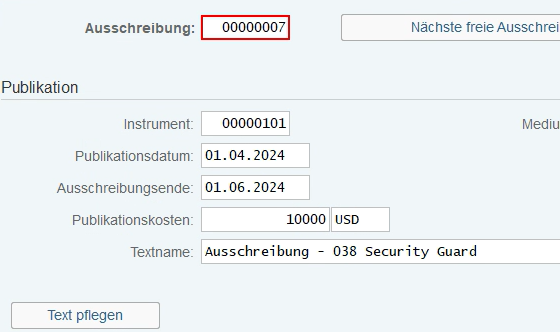
\includegraphics[scale=0.6]{fuellen_ausschreibung}
	\caption{Ausschreibung befüllen}
	\label{fig:fuellen_ausschreibung}
\end{figure}
Als Ausschreibungstext wird folgender Text formuliert:

\textsl{
	Zu Ihren Aufgaben gehört die Überwachung von Gebäuden und Gelände zur Verhinderung von Einbrüchen, Diebstahl und Vandalismus. Sie führen regelmäßige Sicherheitsrundgänge durch, kontrollieren und überwachen den Zugang zu gesicherten Bereichen und überwachen Sicherheitssysteme wie Alarmsysteme und Kameras. Darüber hinaus protokollieren Sie Vorfälle und berichten diese an die Einsatzleitung. In Notfällen leisten Sie Erste Hilfe und arbeiten eng mit Rettungsdiensten und der Polizei zusammen. Ein freundlicher und professioneller Umgang mit Besuchern und Mitarbeitern ist für Sie selbstverständlich.
}

\textsl{
	Sie haben eine abgeschlossene Ausbildung im Sicherheitsbereich oder vergleichbare Qualifikationen sowie einen gültigen Sachkundenachweis gemäß § 34a GewO. Idealerweise verfügen Sie über mehrjährige Berufserfahrung im Sicherheitsdienst. Ein einwandfreies polizeiliches Führungszeugnis, körperliche Fitness und die Bereitschaft zu Schichtarbeit sind für Sie selbstverständlich. Sie zeichnen sich durch ausgeprägtes Verantwortungsbewusstsein und hohe Zuverlässigkeit aus. Gute Deutschkenntnisse in Wort und Schrift sind erforderlich, weitere Sprachkenntnisse sind von Vorteil. Kommunikations- und Teamfähigkeit runden Ihr Profil ab.
}

\textsl{
	Wir bieten Ihnen eine sichere Anstellung in einem wachsenden Unternehmen mit leistungsgerechter Vergütung und attraktiven Zuschlägen für Nacht-, Wochenend- und Feiertagsarbeit. Sie erhalten eine umfassende Einarbeitung und regelmäßige Fort- und Weiterbildungen. Moderne Arbeitskleidung und Ausrüstung stellen wir Ihnen zur Verfügung. Es erwartet Sie ein kollegiales Arbeitsumfeld mit flachen Hierarchien.
}

Danach wird die Planstelle „038 Security Guard“ für die soeben angelegt Ausschreibung hinzugefügt.
\begin{figure}[H]
	\centering
	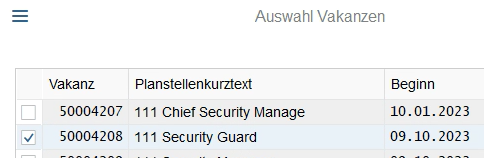
\includegraphics[scale=0.6]{planstelle_ausschreibung}
	\caption{Ausschreibung der Planstelle}
	\label{fig:planstelle_ausschreibung}
\end{figure}

\subsubsection{Erfassen Bewerberdaten}
Um Bewerberdaten zu erfassen, wird die Anwendung „Ersterfassung“ verwendet.
\begin{figure}[H]
	\centering
	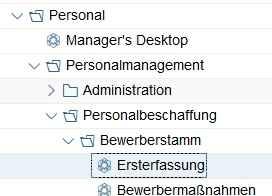
\includegraphics[scale=0.6]{ersterfassung}
	\caption{Pfad Bewerberstamm Ersterfassung}
	\label{fig:ersterfassung}
\end{figure}
Im Bereich Organisatorische Zuordnung wird der Personalbereich „DL00“,  der Personalteilbereich (Pers. suba) „FI00“ und die Bewerbergruppe „1“ definiert. Der Bewerber wird dem Bewerberkreis über die F4-Hilfe Angestellte zugeordnet und der verantwortliche Personalreferent ist „Chris Thomas“. Die Felder Anrede, Name und Geburtsdatum werden mit Daten „Markus“, „Laberuski“ und „01.02.1982“ befüllt und als Sprache wird „EU“ gewählt. Als angelegte Stellenausschreibung wird die „Ausschreibung – 038 Security Guard“ ausgewählt.
\begin{figure}[H]
	\centering
	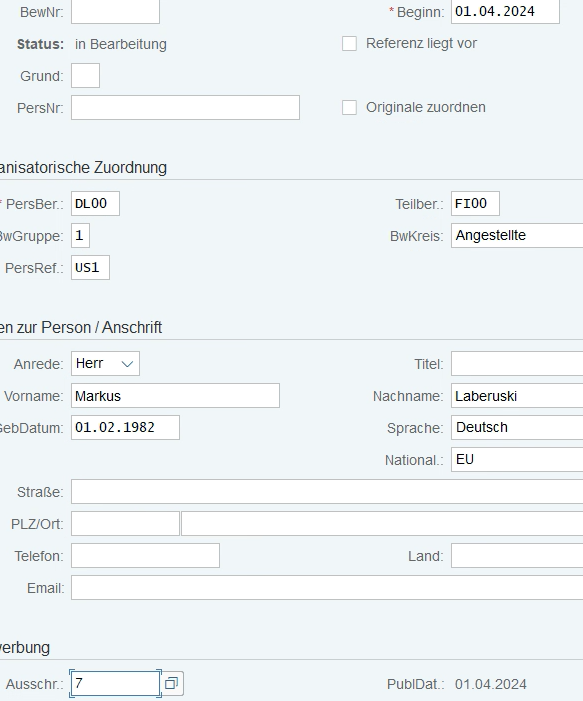
\includegraphics[scale=0.5]{daten_bewerber}
	\caption{Bewerberdaten}
	\label{fig:daten_bewerber}
\end{figure}
Danach öffnet sich das Fenster „Subtypen zum Infotyp Anschrift“, wobei die Anschrift als „Ständiger Wohnsitz“ definiert wird. Im Bild Anschriften anlegen wird die Addressline 1 mit „Ahornsirupweg 402D“ eingegeben, als Ort wird „Dallas“ gewählt und die Postleitzahl mit „75202“ definiert. Der Länderschlüssel wird mit „USA“ gekennzeichnet, sowie der Bundesstaat mit „Texas“ definiert.
\begin{figure}[H]
	\centering
	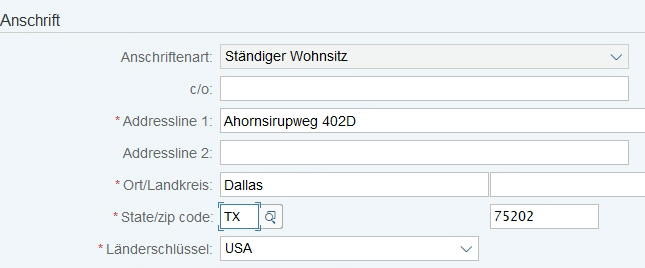
\includegraphics[scale=0.6]{anschrift_markus}
	\caption{Anschrift von Markus}
	\label{fig:anschrift_markus}
\end{figure}
Im darauffolgenden Bild Kommunikation wird als System-ID die fiktive E-Mailadresse markus\_billybilli@web.com erstellt. Nachdem die Daten gesichert werden, gibt SAP die Bewerbernummer „00000012“ in der unteren Statusleiste aus.
\begin{figure}[H]
	\centering
	
\includegraphics[scale=0.6]{bewerbernummer}
	\caption{Bewerbernummer}
	\label{fig:bewerbernummer}
\end{figure}

\subsubsection{Vorbereiten der Einstellung}
Um die Einstellung vorzubereiten, wird die Anwendung „Bewerbermaßnahmen“ verwendet.
\begin{figure}[H]
	\centering
	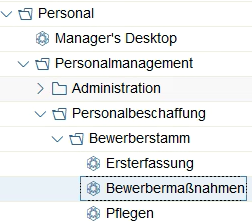
\includegraphics[scale=0.6]{pfad_bewerbermassnahmen}
	\caption{Pfad Bewerbermaßnahmen}
	\label{fig:pfad_bewerbermassnahmen}
\end{figure}
Im Fenster Bewerbermaßnahmen wird die Bewerbernummer „12“ eingegeben und mit Enter bestätigt, um die Bewerberdaten zu laden. Der Bewerber wird zum „01.04.2024“ eingestellt werden. Danach wird die Bewerbermaßnahme „Einstellung vorbereiten“ ausgewählt und ausgeführt.
\begin{figure}[H]
	\centering
	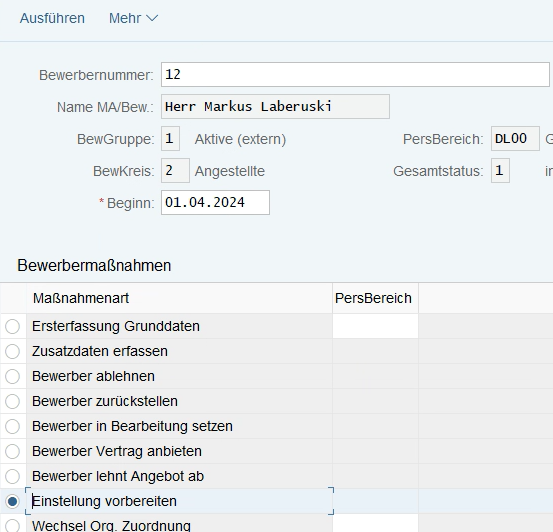
\includegraphics[scale=0.6]{vorbereiten_einstellung}
	\caption{Vorbereiten der Einstellung}
	\label{fig:vorbereiten_einstellung}
\end{figure}
Das Fenster „Bewerbermaßnahme kopieren“ wird mit den vorhandenen Daten gesichert und der Warnhinweis mit Enter bestätigt. Der Warnhinweis, dass der geplante Vorgang in der Zukunft liegt, wird bestätigt und das Fenster „Geplanten Vorgang“ anlegen mit „Übernehmen“ geschlossen.

\subsubsection{Einstellen der Bewerber}
Um einen Bewerber einzustellen wird die Anwendung „Personalmaßnamen“ verwendet.
\begin{figure}[H]
	\centering
	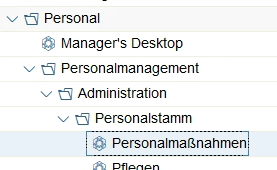
\includegraphics[scale=0.6]{pfad_personalmassnahmen}
	\caption{Pfad Personalmaßnahmen}
	\label{fig:pfad_personalmassnahmen}
\end{figure}
Als Beginn wird der „01.04.2024“ eingegeben und das Feld Personalnummer wird leer gelassen. Anschließend wird die Personalmaßnahme „Einstellung mit Datenübernahme“ ausgewählt und in den daneben liegenden Feldern wird als Personalbereich „DL00“, Mitarbeitergruppe „1“ und Mitarbeiterkreis „U4“ eingegeben.
\begin{figure}[H]
	\centering
	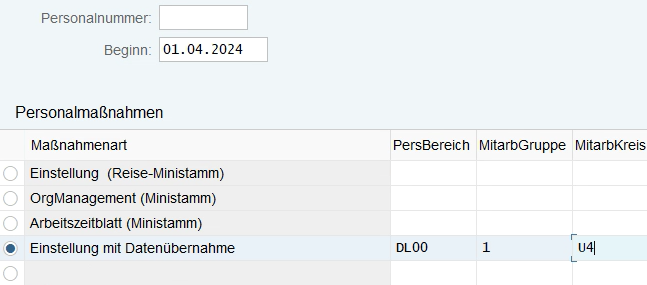
\includegraphics[scale=0.6]{einstellen_bewerber}
	\caption{Bewerber einstellen}
	\label{fig:einstellen_bewerber}
\end{figure}
Im Fenster „Direkte Datenübernahme“ wird die Bewerbernummer „00000012“ eingegeben. Im Fenster „Maßnahmen anlegen“ wird im Feld „Planstelle“ mithilfe der F4-Eingabehilfe die Planstelle „038 Security Guard“ ausgewählt.
\begin{figure}[H]
	\centering
	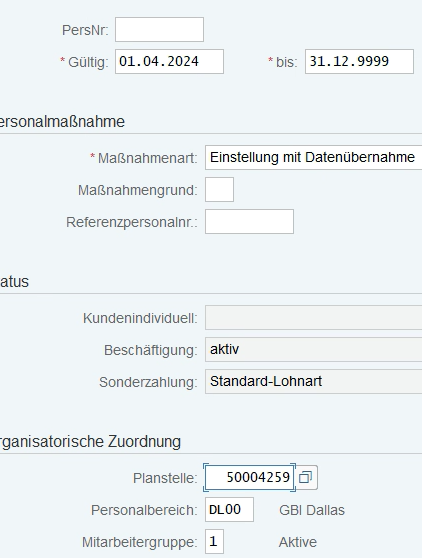
\includegraphics[scale=0.6]{anlegen_massnahme}
	\caption{Maßnahme anlegen}
	\label{fig:anlegen_massnahme}
\end{figure}
Im Bild „Daten zur Person anlegen“ wird die 9-stellige Nummer „918526038“ als Sozialversicherungsnummer (SSN) eingegeben und mit Enter bestätigt. Die restlichen Daten werden aus der Bewerberdatenbank übernommen und können ohne weitere Änderung gesichert werden. Das Bild „Organisatorische Zuordnung anlegen“ wird mit den vorgegebenen Daten gesichert. Die aufkommende Meldung Vakanz abgrenzen wird mit „Ja“ bestätigt. Den folgenden Infotyp „Anschriften anlegen“ wird ohne Änderungen abgesichert. Im folgenden Bild „Steuergebiet“ wird „TX“ als Steuergebiet ausgewählt. Die Gültigkeit wird auf den „01.04.2024“ angepasst und mit Enter bestätigt. Sowohl der Infotyp „Residence Tax Area anlegen“, als auch die beiden folgenden Infotypen werden ohne Änderungen abgesichert. Die Statusleiste zeigt an, dass der Datensatz angelegt wurde.
\begin{figure}[H]
	\centering
	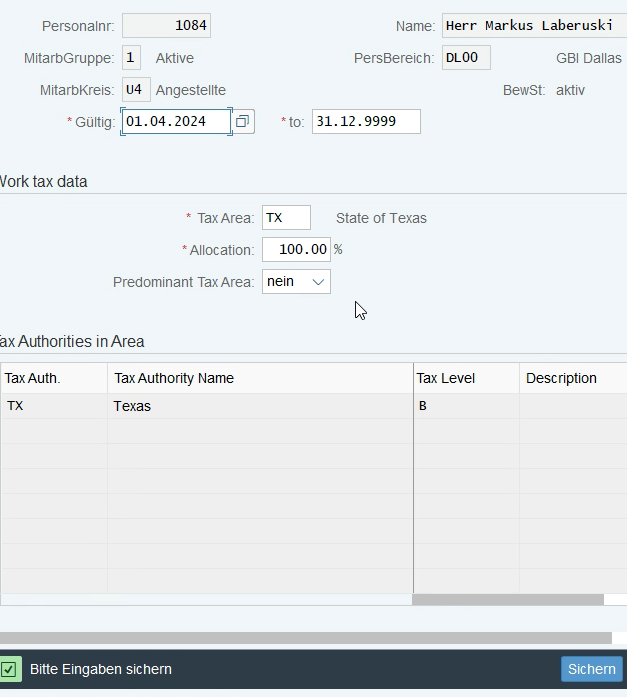
\includegraphics[scale=0.6]{einstellen_bewerber2}
	\caption{Bewerber einstellen 2}
	\label{fig:einstellen_bewerber2}
\end{figure}
Im folgenden Bild „Steuergebiet wählen“ wird „TX“ als Steuergebiet ausgewählt. Alle drei Steueransichten werden mit etwaige Datenüberschreibungen gesichert. Den Infotypen „Bankverbindung anlegen“ wird ohne Änderungen gesichert. Da der Status der Person von Bewerber zum Mitarbeiter erfolgt, wird im Bild „Kommunikation anlegen“ die System-ID auf markus.laberuski@gb.com geändert. Die automatische angelegt Personalnummer ist die „1084“.


\subsection{Personalentwicklung}

\subsubsection{Pflegen des Qualifikationsprofils}
Um ein Qualifikationsprofil zu pflegen, wird die Anwendung „Profil ändern“ verwendet.
\begin{figure}[H]
	\centering
	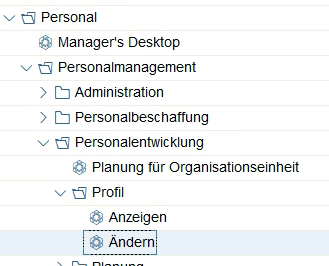
\includegraphics[scale=0.6]{profil_aendern}
	\caption{Profil ändern 2}
	\label{fig:profil_aendern}
\end{figure}
Über die Suche wird der neuangestellte Security Guard „Laberuski“ gefunden und mit einem Doppelklick geöffnet. Es wird eine neue Qualifikation hinzugefügt, indem unter der Tabelle auf „anlegen“ geklickt wird. Im Fenster „Qualifikation“ wird auf den Reiter Struktursuche gewechselt und die „Certification“ expandiert. Es wird nach „First Aid Certification“ selektiert und die Eingabe mit einem Klick auf „Weiter“. Das Datum wird auf den „01.04.2024“ geändert.
\begin{figure}[H]
	\centering
	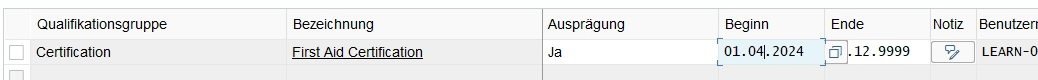
\includegraphics[scale=0.6]{profil_qualifikation}
	\caption{Profil Qualifikationen}
	\label{fig:profil_qualifikation}
\end{figure}

\subsubsection{Durchführen der Laufbahnplanung}
Um eine Laufbahnplanung durchzuführen, wird die Anwendung „Laufbahnplanung“ verwendet.
\begin{figure}[H]
	\centering
	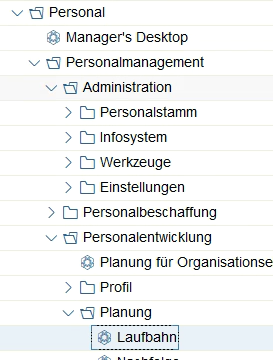
\includegraphics[scale=0.6]{pfad_laufbahnplanung}
	\caption{Pfad Laufbahnplanung}
	\label{fig:pfad_laufbahnplanung}
\end{figure}
Es wird sichergestellt, dass „Person“ gewählt ist. Es wird die Personalnummer „00001084“ für neu eingestellten Security Guard „Markus“ eingegeben. Im Bereich „Auswertungszeitraum“ wird der „16.05.2024“ als Stichtag eingetragen. Als Planungskriterien werden Qualifikationen und Laufbahn markiert.
\begin{figure}[H]
	\centering
	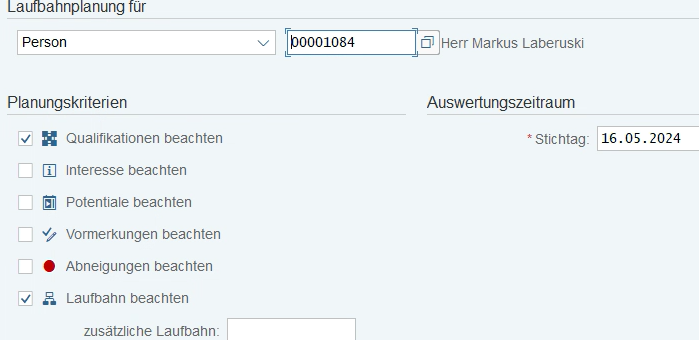
\includegraphics[scale=0.6]{markus_laufbahnplanung}
	\caption{Laufbahnplanung von Markus}
	\label{fig:markus_laufbahnplanung}
\end{figure}
Ihr Mitarbeiter soll für die Planstelle „038 Security Manager“ vorgemerkt werden, da er die Laufbahn „038 Security Guard“ beschreiten soll. Dafür soll die Planstelle aus der Laufbahn aus und abschließend „Mehr, Planung, Anlegen, Vormerkung“ ausgewählt werden. Die Planstelle „038 Security Manager“ kann allerdings nicht ausgewählt werden, weil die Planstelle nicht angezeigt wird. 
\begin{figure}[H]
	\centering
	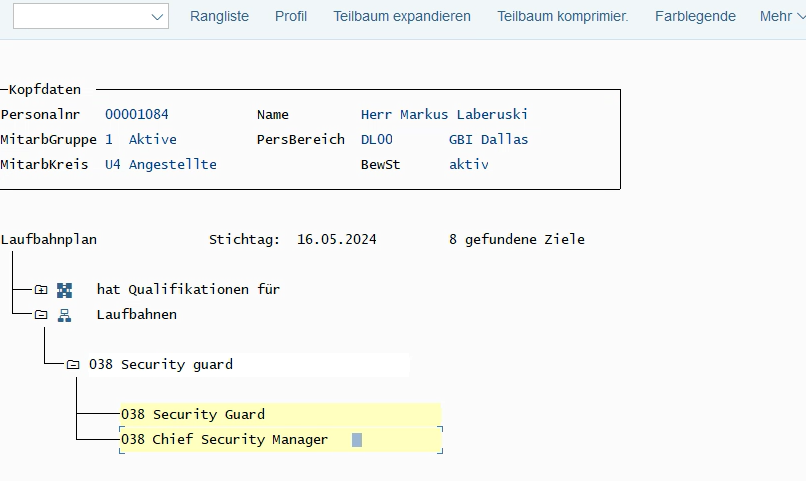
\includegraphics[scale=0.6]{fehlende_planstelle}
	\caption{Fehlende Planstelle}
	\label{fig:fehlende_planstelle}
\end{figure}

\subsubsection{Anlegen der Veranstaltung}
Um eine Veranstaltung anzulegen, wird die Anwendung „Veranstaltungsmenü“ verwendet.
\begin{figure}[H]
	\centering
	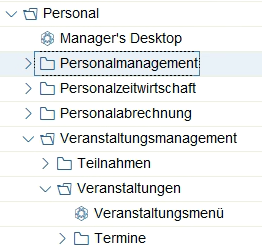
\includegraphics[scale=0.6]{pfad_veranstaltungsmenue}
	\caption{Pfad Veranstaltungsmenü}
	\label{fig:pfad_veranstaltungsmenue}
\end{figure}
Im Bild „Dynamisches Veranstaltungsmenü“ wird das Kontextmenü über einen Rechtsklick geöffnet und „Anlegen ohne Ressourcen“ ausgewählt.
\begin{figure}[H]
	\centering
	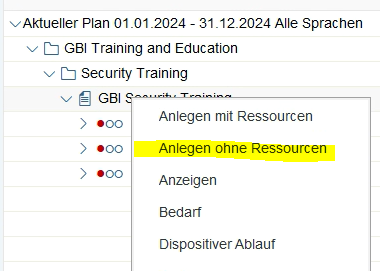
\includegraphics[scale=0.6]{anlegen_ohneressourcen}
	\caption{Veranstaltung anlegen ohne Ressourcen}
	\label{fig:anlegen_ohneressourcen}
\end{figure}
Im folgenden Fenster „Veranstaltung ohne Ressourcen anlegen“ wird als Beginndatum der „06.05.2024“ definiert und Status auf „fixiert“ geändert. Die Bezeichnung der Veranstaltung wird auf „038 ST“ und „038 GBI Sicherheitstraining“ geändert. Als Veranstaltungsort wird über die F4-Eingabehilfe das Schulungszentrum „Dallas“ ausgewählt. Abschließend wird 1 als minimale, optimale und maximale Teilnehmerzahl eingegeben.
\begin{figure}[H]
	\centering
	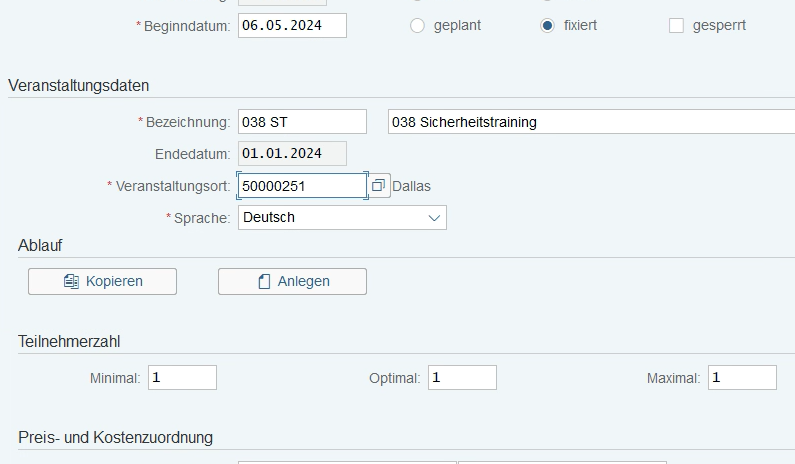
\includegraphics[scale=0.6]{pflege_veranstaltung}
	\caption{Pflege der Veranstaltung}
	\label{fig:pflege_veranstaltung}
\end{figure}
Im aufkommenden Bild „Eigenen Ablauf anlegen“ wird eine Dauer von „3 Tagen“ und „21 Stunden“ im Reiter „Ablauf ohne Muster“ eingegeben. Als Beginntag wird der Montag ausgewählt.
\begin{figure}[H]
	\centering
	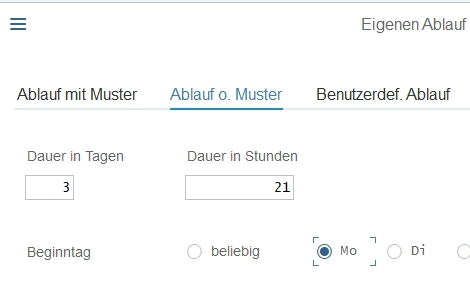
\includegraphics[scale=0.6]{anlegen_ablauf}
	\caption{Ablauf anlegen}
	\label{fig:anlegen_ablauf}
\end{figure}

\subsubsection{Buchen der Veranstaltung}
Um eine Veranstaltung zu buchen, wird die Anwendung „Teilnahmemenü“ verwendet.
\begin{figure}[H]
	\centering
	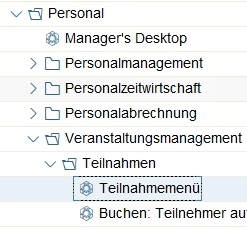
\includegraphics[scale=0.6]{pfad_teilnahmemenue}
	\caption{Pfad Teilnahmemenü}
	\label{fig:pfad_teilnahmemenue}
\end{figure}
Die Veranstaltung wird über den Pfad GBI Training and Education, Security Training, GBI Security Training ausgewählt und mit einem Rechtklick gebucht.
\begin{figure}[H]
	\centering
	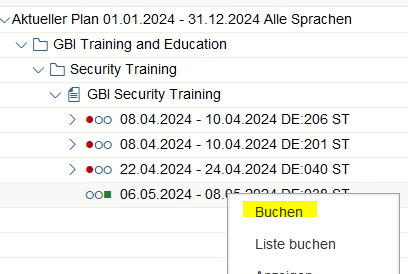
\includegraphics[scale=0.6]{buchen_veranstaltung}
	\caption{Veranstaltung buchen}
	\label{fig:buchen_veranstaltung}
\end{figure}
Im Fenster „Teilnahme buchen“ wird die Personalnummer „00001084“ eingegeben.
\begin{figure}[H]
	\centering
	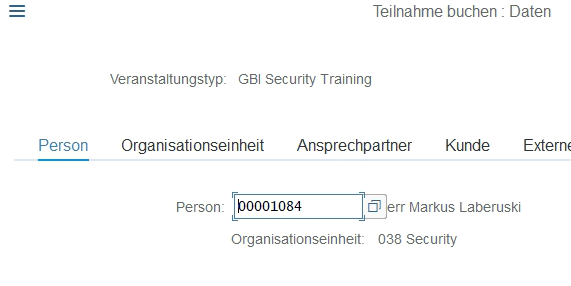
\includegraphics[scale=0.6]{buchen_teilnahme}
	\caption{Teilnahme buchen}
	\label{fig:buchen_teilnahme}
\end{figure}
Es wird die Option „Buchen/Zahlungsinfo“ verwendet und als Abrechnungsart „Gebührenfrei“ ausgewählt. Das Fenster „Gebühr und Zuordnung“ wird anschließend durch „Sichern“ geschlossen. 
\begin{figure}[H]
	\centering
	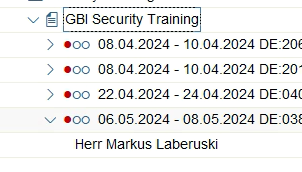
\includegraphics[scale=0.6]{buchen_teilnahme2}
	\caption{Teilnahme buchen 2}
	\label{fig:buchen_teilnahme2}
\end{figure}

\subsubsection{Nachbereiten der Veranstaltung}
Um die Nachbereitung der Veranstaltung durchzuführen, wird die Anwendung „Veranstaltungsmenü“ verwendet.
\begin{figure}[H]
	\centering
	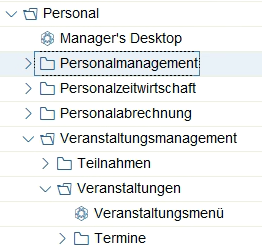
\includegraphics[scale=0.6]{pfad_veranstaltungsmenue}
	\caption{Pfad Veranstaltungsmenü 2}
	\label{fig:pfad_veranstaltungsmenue2}
\end{figure}
Um den Zeitraum der Planvariante zu korrigieren, wird die Menüfunktionsleiste über folgenden Pfad geöffnet: \textit{Mehr-->Einstellungen-->Einstellungen ändern …}. Es wird in den Oberreiter „Dynamische Menüs“ und dort in den Reiter „Veranstaltungsmenüs“ gewechselt. Der Zeitraum wird auf den „01.01.2024“ bis zum „31.12.2024“ und das Datum auf fix definiert.
\begin{figure}[H]
	\centering
	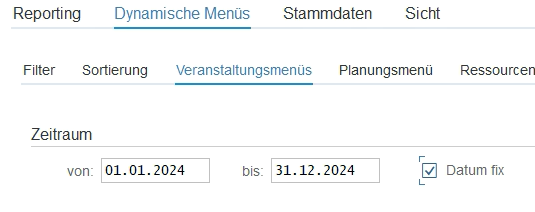
\includegraphics[scale=0.6]{einstellungen_veranstaltung}
	\caption{Veranstaltung Einstellungen}
	\label{fig:einstellungen_veranstaltung}
\end{figure}
In der Veranstaltung wird mit einem Rechtsklick zu „Nachbereiten“ navigiert.
\begin{figure}[H]
	\centering
	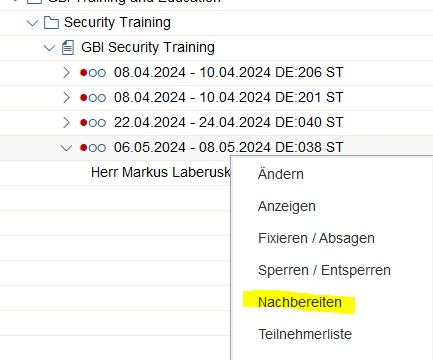
\includegraphics[scale=0.6]{navigieren_nachbereiten}
	\caption{Veranstaltung nachbereiten}
	\label{fig:navigieren_nachbereiten}
\end{figure}
Anschließend wird die Nachbereitung durch Klick auf „Datenbild“ gestartet. Als Ausprägung wird „Ja“ angegeben. Der Mitarbeiter „Markus“ erhält für die Teilnahme ein neues Qualifikationszertifikat.
\begin{figure}[H]
	\centering
	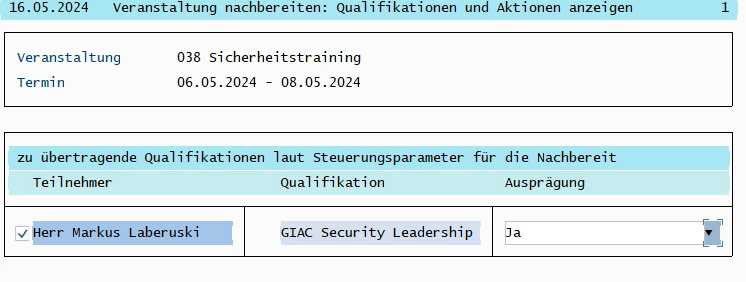
\includegraphics[scale=0.6]{qualifikationszertifikat}
	\caption{Qualifikationszertifikat}
	\label{fig:qualifikationszertifikat}
\end{figure}

\subsubsection{Durchführen der Laufbahnplanung}
Um eine Laufbahnplanung durchzuführen, wird die Anwendung „Laufbahnplanung“ verwendet.
\begin{figure}[H]
	\centering
	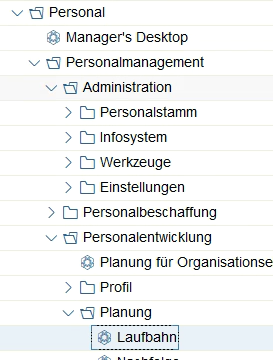
\includegraphics[scale=0.6]{pfad_laufbahnplanung}
	\caption{Pfad Laufbahnplanung 2}
	\label{fig:pfad_laufbahnplanung2}
\end{figure}
Es wird die Personalnummer „0001084“ eingeben. Im Bereich „Auswertungszeitraum“ wird das Datum „16.05.2024“ als Stichtag eingebeben. Als Planungskriterien werden „Qualifikationen“ und „Laufbahn beachtet“ ausgewählt und ausgeführt. Die Planstelle wird allerdings immer noch nicht angezeigt.
\begin{figure}[H]
	\centering
	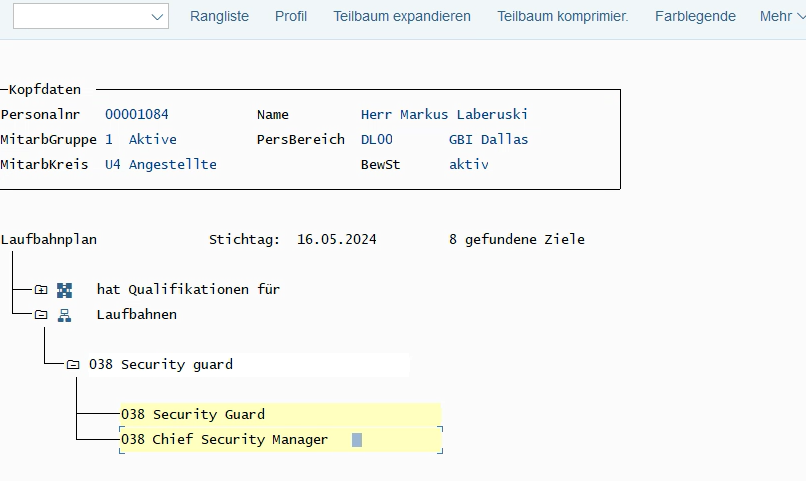
\includegraphics[scale=0.6]{fehlende_planstelle}
	\caption{Fehlende Planstelle 2}
	\label{fig:fehlende_planstelle2}
\end{figure}


\subsection{Beurteilungsprozess}

\subsubsection{Vorbereiten der Beurteilung}
Um eine Beurteilung vorzubereiten, wird die Anwendung „Beurteilung anlegen“ verwendet.
\begin{figure}[H]
	\centering
	\includegraphics[scale=0.6]{pfad_beurteilunganlegen}
	\caption{Pfad Beurteilung anlegen}
	\label{fig:pfad_beurteilunganlegen}
\end{figure}
Es wird das Beurteilungsformular „Individual Performance Appraisal“ ausgewählt. Es wird vom „16.05.2024“ bis zum „16.06.2024“ gültig sein. Um zu definieren, wer eine Beurteilung abgibt, wird der Vorgesetzter ausgewählt und die Mitarbeiterin „Sabine Matoschek“, die die Stelle des „038 Chief Security Managers“ belegt, gesucht. Daraufhin wird der „Arbeitsvorrat“ angezeigt, welcher alle Mitarbeiter enthält, für die der Vorgesetzte eine Beurteilung abgeben kann.
\begin{figure}[H]
	\centering
	\includegraphics[scale=0.6]{auswahl_arbeitsvorrat}
	\caption{Auswahl Arbeitsvorrat}
	\label{fig:auswahl_arbeitsvorrat}
\end{figure}
Es wird der Mitarbeiter „Markus“ ausgewählt und „Vorbereitung abschließen“ gedrückt, um die Planung der Beurteilung zu beenden. In der Statusleiste wird folgende Meldung ausgegeben:
\begin{figure}[H]
	\centering
	\includegraphics[scale=0.6]{status_geaendert}
	\caption{Status geändert}
	\label{fig:status_geaendert}
\end{figure}

\subsubsection{Durchführen der Beurteilung}
Um die Beurteilung durchzuführen, wird die Anwendung „Beurteilung bearbeiten“ verwendet.
\begin{figure}[H]
	\centering
	\includegraphics[scale=0.6]{pfad_beurteilungbearbeiten}
	\caption{Pfad Beurteilung bearbeiten}
	\label{fig:pfad_beurteilungbearbeiten}
\end{figure}
Im Bild „Beurteilung“ wird das Beurteilungsmuster „Individual Performance Appraisal“ mit der F4-Hilfe ausgewählt. Der Beurteilungszeitraum wird vom „16.05.2024“ bis zum „16.06.2024“ definiert. Im Bereich „Beteiligte“ für die „Beurteiler Person“ wird die die Mitarbeiterin „Sabine“ ausgewählt. Für die „Beurteilte Person“ wird der Mitarbeiter „Markus“ ausgewählt. Danach wird der Beurteilungsstatus „In Bearbeitung“ selektiert und „Durchführen“ gewählt.
\begin{figure}[H]
	\centering
	\includegraphics[scale=0.6]{bearbeiten_beurteilung}
	\caption{Beurteilung bearbeiten}
	\label{fig:bearbeiten_beurteilung}
\end{figure}
Es wird auf die Funktion „Ändern“ gedrückt. Im folgenden Bild „Beurteilung durchführen“ werden die Ziele angezeigt, die der Mitarbeiter erreichen soll.
\begin{figure}[H]
	\centering
	\includegraphics[scale=0.6]{ziele_beurteilung}
	\caption{Beurteilungsziele}
	\label{fig:ziele_beurteilung}
\end{figure}

\subsubsection{Versetzen der Mitarbeiter}
Um einen Mitarbeiter zu versetzen, wird die Anwendung „Organisation und Besetzung ändern“ verwendet.
\begin{figure}[H]
	\centering
	\includegraphics[scale=0.6]{pfad_organisationundbesetzungaendern}
	\caption{Pfad Organisation und Besetzung ändern}
	\label{fig:pfad_organisationundbesetzungaendern}
\end{figure}
In der Abbildung 58 wird der Besetzungsplan der „038 Security“ Abteilung dargestellt. Die Besetzung des Mitarbeiters „Markus“ wird geändert, indem der Mitarbeiter per Drag \& Drop auf die vakante Planstelle des Security Managers gezogen wird.
\begin{figure}[H]
	\centering
	\includegraphics[scale=0.6]{orga_besetzung}
	\caption{Besetzungsplan der Organisation}
	\label{fig:orga_besetzung}
\end{figure}
Der Dialog „Person zuordnen“ wird geöffnet. Es wird der „01.05.2024“ als Gültig vom und „100\%“ als Besetzungsprozentsatz eingegeben. Der Stellenumsetzung wird als Maßnahme ausgewählt. Es wird die Planstelle des Security Guards selektiert, um die Verknüpfung gänzlich zu terminieren.
\begin{figure}[H]
	\centering
	\includegraphics[scale=0.6]{stellenumsetzung}
	\caption{Stellenumsetzung}
	\label{fig:stellenumsetzung}
\end{figure}
Die Planstelle des Security Guards wird auf das Datum „16.05.2024“ wieder vakant gesetzt. Zusätzlich wird die Planstelle des Security Managers zum „01.05.2024“ abgegrenzt.
\begin{figure}[H]
	\centering
	\includegraphics[scale=0.6]{neuerbesetzungsplan}
	\caption{Neuer Besetzungsplan}
	\label{fig:neuerbesetzungsplan}
\end{figure}
\clearpage